% Options for packages loaded elsewhere
\PassOptionsToPackage{unicode}{hyperref}
\PassOptionsToPackage{hyphens}{url}
%
\documentclass[
]{article}
\usepackage{amsmath,amssymb}
\usepackage{lmodern}
\usepackage{iftex}
\ifPDFTeX
  \usepackage[T1]{fontenc}
  \usepackage[utf8]{inputenc}
  \usepackage{textcomp} % provide euro and other symbols
\else % if luatex or xetex
  \usepackage{unicode-math}
  \defaultfontfeatures{Scale=MatchLowercase}
  \defaultfontfeatures[\rmfamily]{Ligatures=TeX,Scale=1}
\fi
% Use upquote if available, for straight quotes in verbatim environments
\IfFileExists{upquote.sty}{\usepackage{upquote}}{}
\IfFileExists{microtype.sty}{% use microtype if available
  \usepackage[]{microtype}
  \UseMicrotypeSet[protrusion]{basicmath} % disable protrusion for tt fonts
}{}
\makeatletter
\@ifundefined{KOMAClassName}{% if non-KOMA class
  \IfFileExists{parskip.sty}{%
    \usepackage{parskip}
  }{% else
    \setlength{\parindent}{0pt}
    \setlength{\parskip}{6pt plus 2pt minus 1pt}}
}{% if KOMA class
  \KOMAoptions{parskip=half}}
\makeatother
\usepackage{xcolor}
\IfFileExists{xurl.sty}{\usepackage{xurl}}{} % add URL line breaks if available
\IfFileExists{bookmark.sty}{\usepackage{bookmark}}{\usepackage{hyperref}}
\hypersetup{
  pdftitle={Data Analysis Coursebook},
  pdfauthor={Marcell Granat \& Zoltan Madari},
  hidelinks,
  pdfcreator={LaTeX via pandoc}}
\urlstyle{same} % disable monospaced font for URLs
\usepackage[margin=1in]{geometry}
\usepackage{color}
\usepackage{fancyvrb}
\newcommand{\VerbBar}{|}
\newcommand{\VERB}{\Verb[commandchars=\\\{\}]}
\DefineVerbatimEnvironment{Highlighting}{Verbatim}{commandchars=\\\{\}}
% Add ',fontsize=\small' for more characters per line
\usepackage{framed}
\definecolor{shadecolor}{RGB}{248,248,248}
\newenvironment{Shaded}{\begin{snugshade}}{\end{snugshade}}
\newcommand{\AlertTok}[1]{\textcolor[rgb]{0.94,0.16,0.16}{#1}}
\newcommand{\AnnotationTok}[1]{\textcolor[rgb]{0.56,0.35,0.01}{\textbf{\textit{#1}}}}
\newcommand{\AttributeTok}[1]{\textcolor[rgb]{0.77,0.63,0.00}{#1}}
\newcommand{\BaseNTok}[1]{\textcolor[rgb]{0.00,0.00,0.81}{#1}}
\newcommand{\BuiltInTok}[1]{#1}
\newcommand{\CharTok}[1]{\textcolor[rgb]{0.31,0.60,0.02}{#1}}
\newcommand{\CommentTok}[1]{\textcolor[rgb]{0.56,0.35,0.01}{\textit{#1}}}
\newcommand{\CommentVarTok}[1]{\textcolor[rgb]{0.56,0.35,0.01}{\textbf{\textit{#1}}}}
\newcommand{\ConstantTok}[1]{\textcolor[rgb]{0.00,0.00,0.00}{#1}}
\newcommand{\ControlFlowTok}[1]{\textcolor[rgb]{0.13,0.29,0.53}{\textbf{#1}}}
\newcommand{\DataTypeTok}[1]{\textcolor[rgb]{0.13,0.29,0.53}{#1}}
\newcommand{\DecValTok}[1]{\textcolor[rgb]{0.00,0.00,0.81}{#1}}
\newcommand{\DocumentationTok}[1]{\textcolor[rgb]{0.56,0.35,0.01}{\textbf{\textit{#1}}}}
\newcommand{\ErrorTok}[1]{\textcolor[rgb]{0.64,0.00,0.00}{\textbf{#1}}}
\newcommand{\ExtensionTok}[1]{#1}
\newcommand{\FloatTok}[1]{\textcolor[rgb]{0.00,0.00,0.81}{#1}}
\newcommand{\FunctionTok}[1]{\textcolor[rgb]{0.00,0.00,0.00}{#1}}
\newcommand{\ImportTok}[1]{#1}
\newcommand{\InformationTok}[1]{\textcolor[rgb]{0.56,0.35,0.01}{\textbf{\textit{#1}}}}
\newcommand{\KeywordTok}[1]{\textcolor[rgb]{0.13,0.29,0.53}{\textbf{#1}}}
\newcommand{\NormalTok}[1]{#1}
\newcommand{\OperatorTok}[1]{\textcolor[rgb]{0.81,0.36,0.00}{\textbf{#1}}}
\newcommand{\OtherTok}[1]{\textcolor[rgb]{0.56,0.35,0.01}{#1}}
\newcommand{\PreprocessorTok}[1]{\textcolor[rgb]{0.56,0.35,0.01}{\textit{#1}}}
\newcommand{\RegionMarkerTok}[1]{#1}
\newcommand{\SpecialCharTok}[1]{\textcolor[rgb]{0.00,0.00,0.00}{#1}}
\newcommand{\SpecialStringTok}[1]{\textcolor[rgb]{0.31,0.60,0.02}{#1}}
\newcommand{\StringTok}[1]{\textcolor[rgb]{0.31,0.60,0.02}{#1}}
\newcommand{\VariableTok}[1]{\textcolor[rgb]{0.00,0.00,0.00}{#1}}
\newcommand{\VerbatimStringTok}[1]{\textcolor[rgb]{0.31,0.60,0.02}{#1}}
\newcommand{\WarningTok}[1]{\textcolor[rgb]{0.56,0.35,0.01}{\textbf{\textit{#1}}}}
\usepackage{longtable,booktabs,array}
\usepackage{calc} % for calculating minipage widths
% Correct order of tables after \paragraph or \subparagraph
\usepackage{etoolbox}
\makeatletter
\patchcmd\longtable{\par}{\if@noskipsec\mbox{}\fi\par}{}{}
\makeatother
% Allow footnotes in longtable head/foot
\IfFileExists{footnotehyper.sty}{\usepackage{footnotehyper}}{\usepackage{footnote}}
\makesavenoteenv{longtable}
\usepackage{graphicx}
\makeatletter
\def\maxwidth{\ifdim\Gin@nat@width>\linewidth\linewidth\else\Gin@nat@width\fi}
\def\maxheight{\ifdim\Gin@nat@height>\textheight\textheight\else\Gin@nat@height\fi}
\makeatother
% Scale images if necessary, so that they will not overflow the page
% margins by default, and it is still possible to overwrite the defaults
% using explicit options in \includegraphics[width, height, ...]{}
\setkeys{Gin}{width=\maxwidth,height=\maxheight,keepaspectratio}
% Set default figure placement to htbp
\makeatletter
\def\fps@figure{htbp}
\makeatother
\setlength{\emergencystretch}{3em} % prevent overfull lines
\providecommand{\tightlist}{%
  \setlength{\itemsep}{0pt}\setlength{\parskip}{0pt}}
\setcounter{secnumdepth}{5}
\usepackage{pdfpages}

\usepackage{booktabs}
\usepackage{amsthm}
\makeatletter
\def\thm@space@setup{%
  \thm@preskip=8pt plus 2pt minus 4pt
  \thm@postskip=\thm@preskip
}
\makeatother


% sidebar environment
\usepackage{framed,color}
\definecolor{shadecolor}{RGB}{242,242,242}
\makeatletter
\newenvironment{sidebar}{%
\medskip{}
\setlength{\fboxsep}{.8em}
 \def\at@end@of@kframe{}%
 \ifinner\ifhmode%
  \def\at@end@of@kframe{\end{minipage}}%
  \begin{minipage}{\columnwidth}%
 \fi\fi%
 \def\FrameCommand##1{\hskip\@totalleftmargin \hskip-\fboxsep
 \colorbox{shadecolor}{##1}\hskip-\fboxsep
     % There is no \\@totalrightmargin, so:
     \hskip-\linewidth \hskip-\@totalleftmargin \hskip\columnwidth}%
 \MakeFramed {\advance\hsize-\width
   \@totalleftmargin\z@ \linewidth\hsize
   \@setminipage}}%
 {\par\unskip\endMakeFramed%
 \at@end@of@kframe}
\makeatother
\ifLuaTeX
  \usepackage{selnolig}  % disable illegal ligatures
\fi
\usepackage[]{natbib}
\bibliographystyle{plainnat}

\title{\textbf{Data Analysis} Coursebook}
\author{Marcell Granat \& Zoltan Madari}
\date{}

\begin{document}
\maketitle

{
\setcounter{tocdepth}{2}
\tableofcontents
}
\pagebreak

\hypertarget{welcome}{%
\section*{Welcome}\label{welcome}}
\addcontentsline{toc}{section}{Welcome}

\emph{I hope this message finds you well.}

This is an online bookdown file, which we plan to \emph{update regularly} with the class material. We suggest that you to write the code simultaneously with us at seminar, but bugs can always occur out of the blue\ldots{} If you missed something or just want to revisit the topic with additional comments (probably before the exam day) this page is here to help.

At the end of the course you should know:

\begin{itemize}
\item
  What are data types, data quality, and data preprocessing?
\item
  What are the components of \texttt{tidyverse} and what are their advantage?
\item
  What are density, distribution function, quantile functions?
\item
  What are data clustering techniques?
\item
  What are the main techniques for association analysis?
\end{itemize}

We will work with \texttt{R}, one the most loved statistical programming language. Do not be afraid if you do not have any programming experience, this is a beginner course. However, by the end of the program, we hope you will find useful the concept and practical tips we offer, and you will be able to solve your own real life data analysis issues.

\hypertarget{syllabus}{%
\section*{Syllabus}\label{syllabus}}
\addcontentsline{toc}{section}{Syllabus}

\hypertarget{topics}{%
\subsection{Topics}\label{topics}}

\begin{itemize}
\item
  \textbf{Basic R knowledge (Week 1)}

  \begin{itemize}
  \item
    Data categorize, sampling, importing-exporting
  \item
    Types, tables, selection, objects, functions
  \end{itemize}
\item
  \textbf{Data manipulation in Tidyverse (Week 2)}

  \begin{itemize}
  \item
    Filter, group\_by, arrange, summarize commands
  \item
    \texttt{\%\textbackslash{}\textgreater{}\%}
  \item
    Join (mutating, filtering)
  \item
    tidy data (longer, wider)
  \end{itemize}
\item
  \textbf{Visualization with ggplot2 (Week 3)}

  \begin{itemize}
  \item
    Layers, facets, geoms
  \item
    Descriptive statistics in R
  \item
    Summary statistics, variability, correlation, covariance
  \item
    Extreme values, problem of missing values
  \end{itemize}
\item
  \textbf{Statistical estimation (Week 4)}

  \begin{itemize}
  \tightlist
  \item
    Distributions
  \item
    Sample techniques, confidence intervals, standard error
  \end{itemize}
\item
  \textbf{Hypothesis testing I (Week 5)}

  \begin{itemize}
  \item
    Inductive statistics in R
  \item
    Null and alternative hypothesis, t-test, p-value, fals
    positive/negative, Type I and II error
  \end{itemize}
\item
  \textbf{Hypothesis testing II (Week 6)}

  \begin{itemize}
  \tightlist
  \item
    Relation testing in R
  \end{itemize}
\item
  \textbf{Project presentations (Week 7)}
\end{itemize}

\hypertarget{requirements}{%
\subsection{\texorpdfstring{\textbf{Requirements}}{Requirements}}\label{requirements}}

\begin{itemize}
\item
  \textbf{Test} (30\%): 90 min task solution in R + explanation (exam week)
\item
  \textbf{Project} (25\%): groups (3-4 students), one detailed report
  (essay) and one - \textbf{presentation}
\item
  \textbf{Homeworks} and essays (45\%)
\item
  \textbf{Extra} tasks (+5\%)
\end{itemize}

\hypertarget{project}{%
\subsubsection{Project}\label{project}}

By the end of the course you have to make a statistical report about your own research project in small groups. You have to find a proper dataset (kaggle, eurostat, UCI datasets etc.) or conduct an own survey in optional topic.

At week 7 you will hold a presentation about your findings and results. At the end of the week you will upload your detailed essay about your project work.

\hypertarget{homework}{%
\subsubsection{Homework}\label{homework}}

During the Study period you get 3-5 homeworks. The number of homeworks depends ont he material progress. It could be R code writing or R code writing and analysis (short essay about methods and results).

\begin{longtable}[]{@{}ll@{}}
\caption{Grades}\tabularnewline
\toprule
\endhead
0-50\% & Fail (1) \\
51-62\% & Pass (2) \\
63-74\% & Satisfactory (3) \\
75-86\% & Good (4) \\
87-100\% & excellent (5) \\
\bottomrule
\end{longtable}

\hypertarget{recommended-compulsory-reading}{%
\subsection{Recommended (compulsory) reading}\label{recommended-compulsory-reading}}

\begin{itemize}
\item
  \href{http://r4ds.had.co.nz/}{\textbf{Grolemund G \& Wickham H:
  R for Data Science}}
\item
  Gábor Békés \& Gábor Kézdi: Data Analysis:
  Patterns, Prediction and Causality
\end{itemize}

\hypertarget{part-week-1}{%
\part*{Week 1}\label{part-week-1}}
\addcontentsline{toc}{part}{Week 1}

\hypertarget{lecture1}{%
\section{Lecture 1}\label{lecture1}}

\hypertarget{seminar1}{%
\section{Introduction to R}\label{seminar1}}

\hypertarget{why-r}{%
\subsection{Why R?}\label{why-r}}

In this chapter we will discuss the basics of R programming.
R is a free software, used by millions in the field of statistics, data science, economics and many others.

\href{https://www.facebook.com/Rmemes0/photos/a.1230204967031792/2971372822914989/}{
\includegraphics[width=6.25in,height=\textheight]{images/meme_free.jpg}}

The R programming language is an important tool for data related tasks, but it is much more.
Just like other programming languages, R has many additional packages, which can extend its basic functionality.
R has a great (probably the best) graphical tools to create your charts, and with shiny, you can easily build your minimalist web applications.
We will learn about data manipulation, analysis and how to create awesome reports, like dashboards.

\hypertarget{layout}{%
\subsection{Setup}\label{layout}}

You can download R and RStudio from the official site of \href{https://www.rstudio.com/products/rstudio/download/\#download}{RStudio}.
Please install the appropriate version based on your OS, and do not forget that you also have to install R as well.

\href{https://www.rstudio.com/products/rstudio/download/\#download}{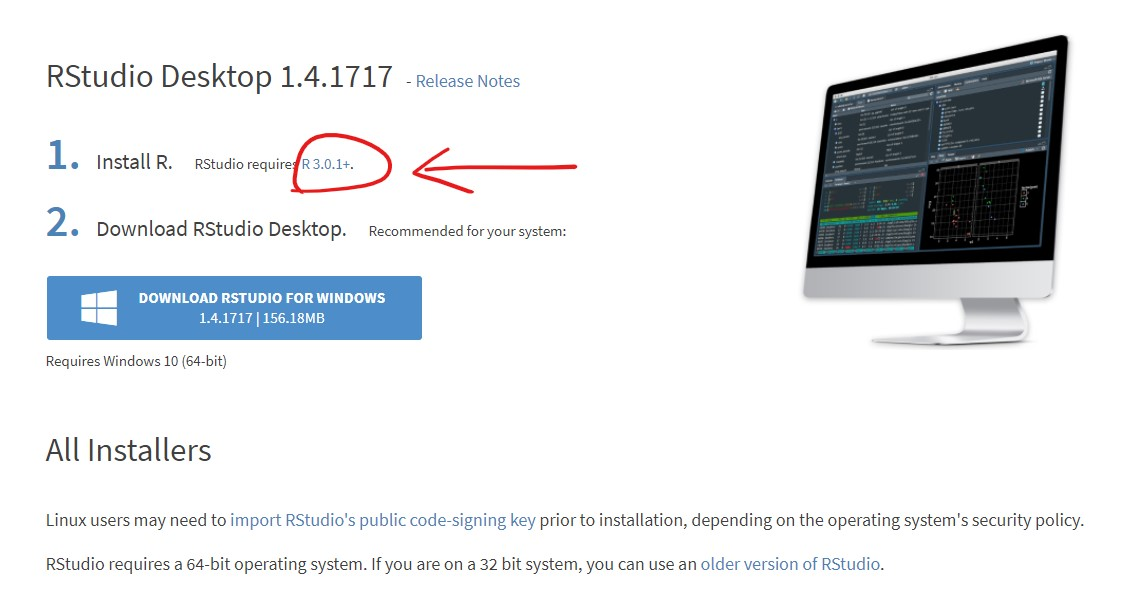
\includegraphics[width=6.25in,height=\textheight]{images/installr.jpg}}

\href{https://cran.rstudio.com/}{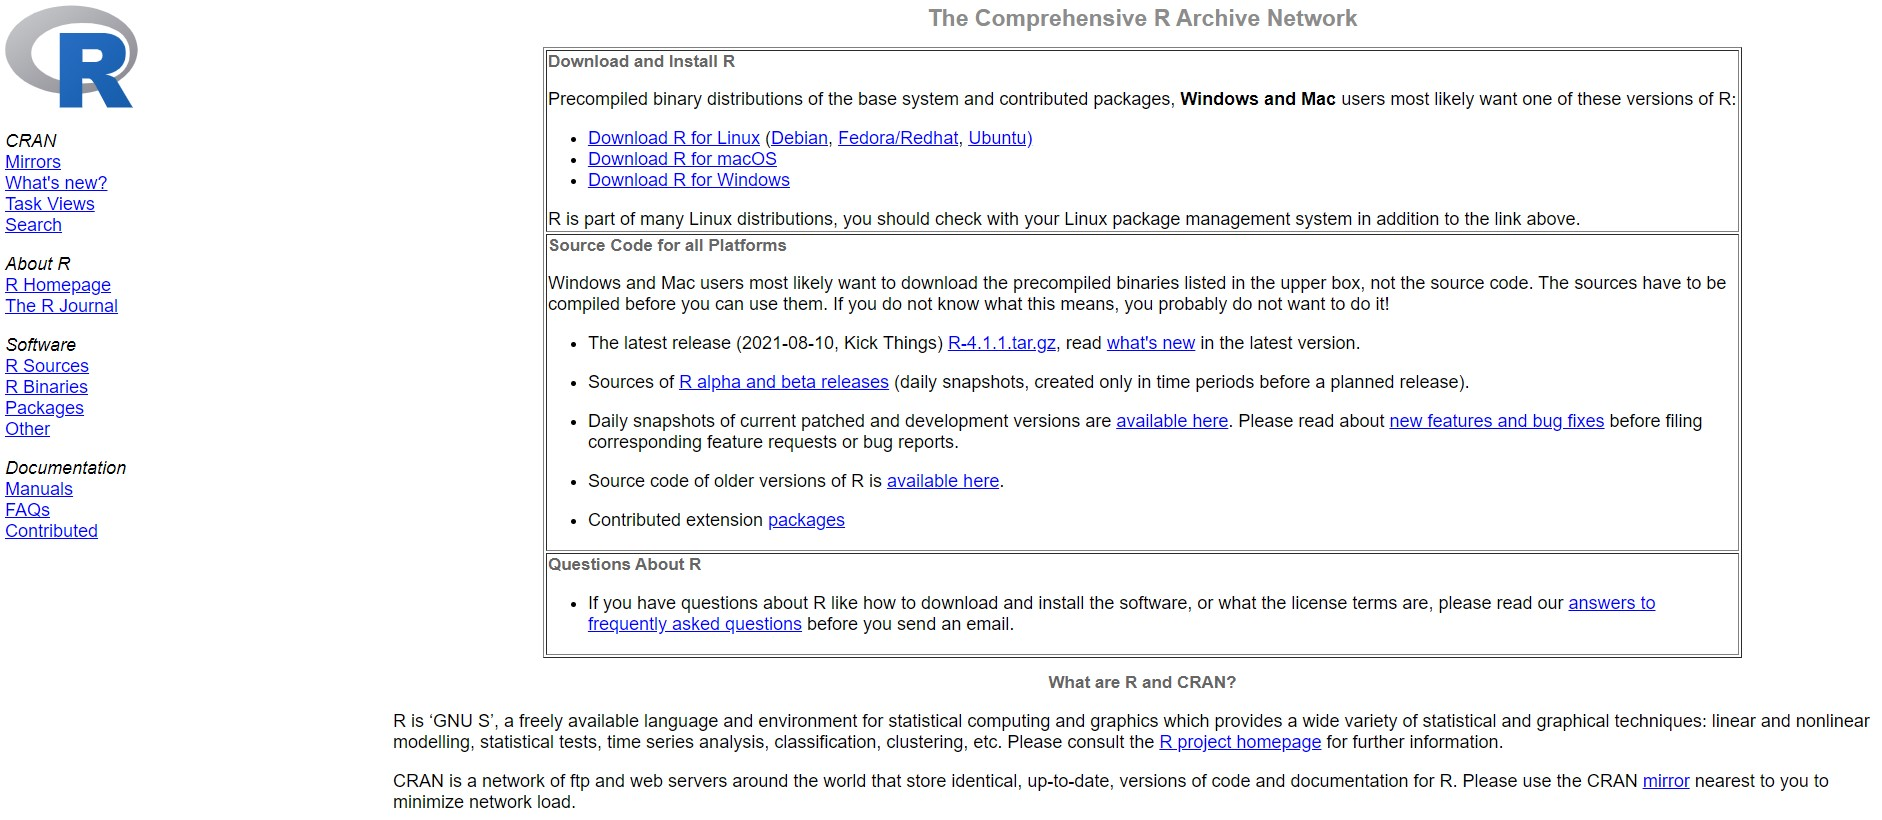
\includegraphics[width=6.25in,height=\textheight]{images/installr2.jpg}}

Run R's installer file after the downloading process is finished.
Next, we will also need the RStudio.

\href{https://www.rstudio.com/products/rstudio/download/\#download}{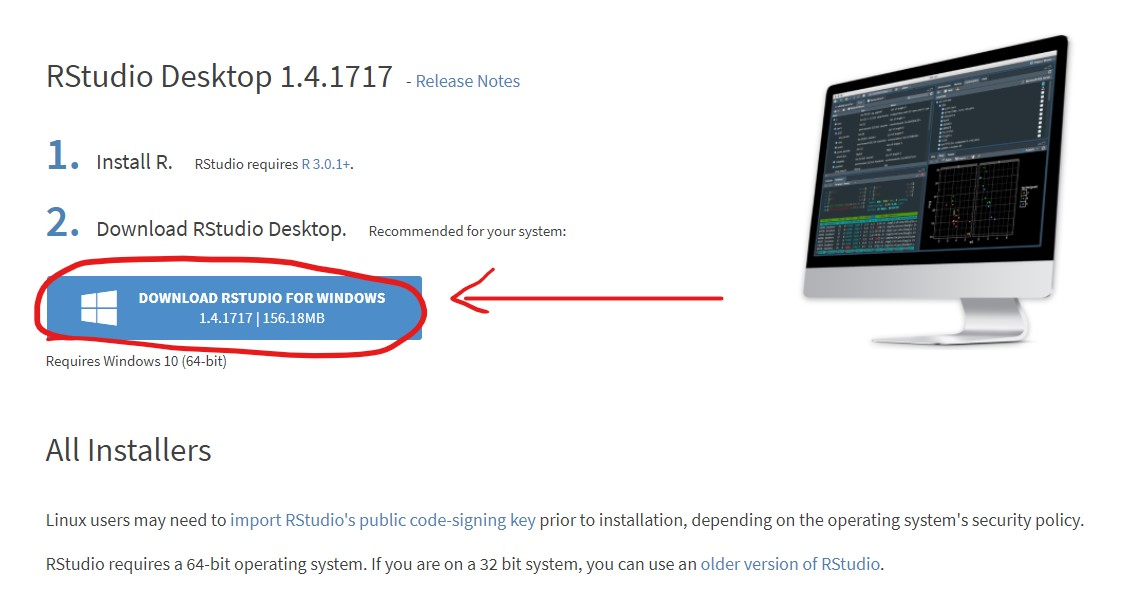
\includegraphics[width=6.25in,height=\textheight]{images/installr3.jpg}}

If the installation process of R and RStudio is finished, then we can open RStudio and start to learn the software.

\hypertarget{our-first-meet-with-r}{%
\subsection{Our first meet with R}\label{our-first-meet-with-r}}

RStudio is dedicated IDEE for R, which means, that it will make our life much simplier.
In stead of writing each line of code ourself, RStudio has many built-in functions to help us.
We see some panes if we open RStudio:

\begin{figure}

{\centering 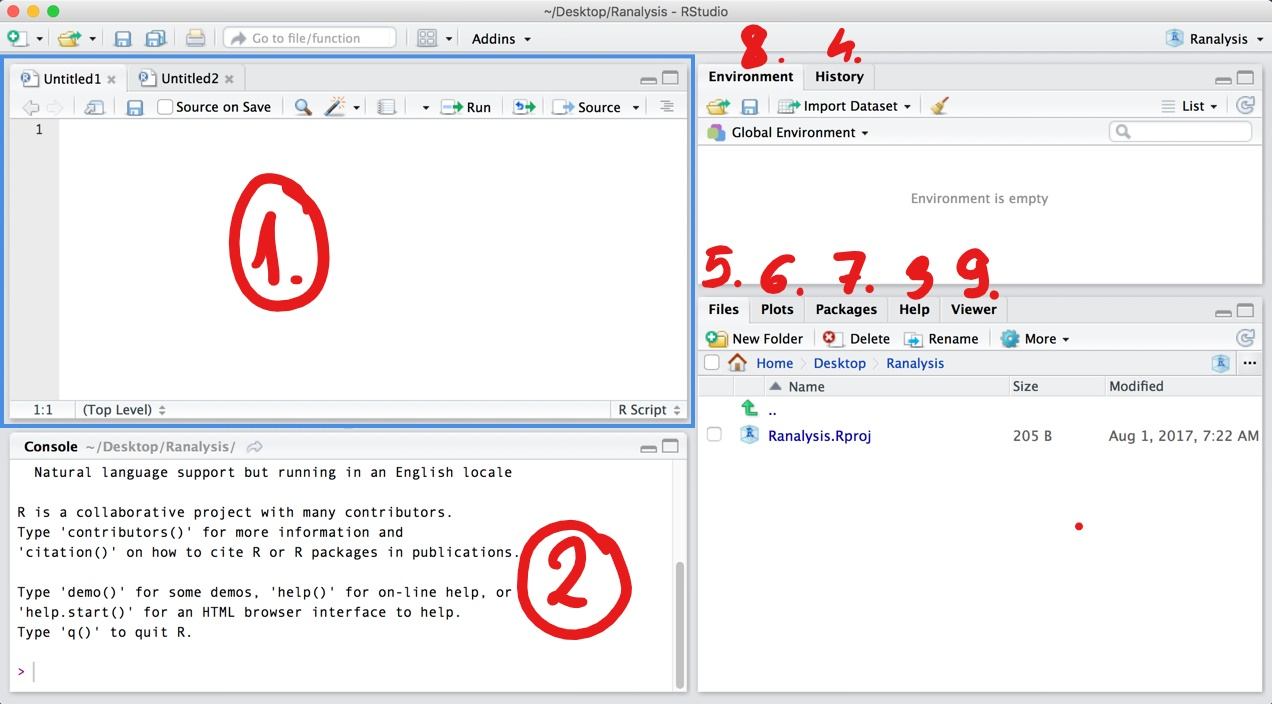
\includegraphics[width=0.7\linewidth]{C:/rprojects/Data-Analysis/images/Inkedrstudio_LI} 

}

\caption{Panes in RStudio}\label{fig:unnamed-chunk-3}
\end{figure}

\begin{enumerate}
\def\labelenumi{\arabic{enumi}.}
\item
  Source

  \begin{itemize}
  \tightlist
  \item
    We will write here our codes, which we would like to save.
    The basic extension of our codes are \texttt{.R}, but this is not the only possibility (we will cover this later). Once you save your code for later use, you can open your script also with a simple text editor (like Notepad), since this is only plain text. If you hit \texttt{enter} your code wont be executed, you will just simply start a new line. If you want to run your code hit \texttt{ctrl\ +\ enter} to execute a single line, and \texttt{ctrl+shift+enter} to execute your full script.
  \end{itemize}
\item
  Console

  \begin{itemize}
  \tightlist
  \item
    Here you find the executed codes, and the response to that. For example, if you type \texttt{2\ +\ 2} and hit \texttt{enter}, R will execute the expression, and response that it is 4.
  \end{itemize}
\end{enumerate}

\begin{Shaded}
\begin{Highlighting}[]
\DecValTok{2} \SpecialCharTok{+} \DecValTok{2}
\CommentTok{\#\textgreater{} [1] 4}
\end{Highlighting}
\end{Shaded}

\begin{enumerate}
\def\labelenumi{\arabic{enumi}.}
\setcounter{enumi}{2}
\item
  Help

  \begin{itemize}
  \tightlist
  \item
    You can use this pane if you are not familier with a function. For example, you want to know what input you can specify while using \texttt{mean}, you can type \texttt{?mean} on the console, or use the search field on this pane. The description of the function will be presented on this pane. (This pane is super useful on the exam)
  \end{itemize}
\item
  History
\item
  Files

  \begin{itemize}
  \tightlist
  \item
    You can see the list of your files which are in the current working directory. Working directory is the folder, from where R want currently read the files. If you want to import a dataset, just click on a file on this pane.
  \item
    I highly recommend you to set a project folder for the class and any later job. This means that, R creates a folder and puts an \texttt{.Rproj} file into it. You can always click on this \texttt{.Rproj} file to return your unfinished work. You can customise if R should put the variables into your environtent as you left them last time, you have a history about the used codes, and you see all the data you copy + paste into this folder.
  \end{itemize}
\item
  Plots
\item
  Packages

  \begin{itemize}
  \tightlist
  \item
    You can install packages from this pane. If you need a given package, click on install, and start typing its name. After that, you have to activate packages each time you open R again with the \texttt{library(eurostat)} command. You can also use a function from a package if you just simly type \texttt{eurostat::get\_eurostat()}.
  \end{itemize}
\item
  Environment

  \begin{itemize}
  \tightlist
  \item
    Here you can see the list of the variables you have already created. For example you can type \texttt{x\ =\ 3} on the console. Now and x variable will appear in the environment pane, and you can check its value if you type \texttt{x} on the console. You can also save these variables into an \texttt{.RData} data format if you wish.
  \end{itemize}
\item
  Viewer
\end{enumerate}

\hypertarget{data-types}{%
\subsection{Data types}\label{data-types}}

Lets see first, what kind of datatypes exist in R. Lets assign a variable called \texttt{x}.

\begin{Shaded}
\begin{Highlighting}[]
\NormalTok{x }\OtherTok{\textless{}{-}} \DecValTok{4}
\end{Highlighting}
\end{Shaded}

So, what is the type of \texttt{x}? We can use the \texttt{class} command to answer this.

\begin{Shaded}
\begin{Highlighting}[]
\FunctionTok{class}\NormalTok{(x)}
\CommentTok{\#\textgreater{} [1] "numeric"}
\end{Highlighting}
\end{Shaded}

Its numeric\footnote{Integer and double also exist in R, but these are not the default, and variables will be always coerced automatically}. This means that you can use \texttt{+}, \texttt{-}, \texttt{*} operators on it.

Lets see other types.

\begin{Shaded}
\begin{Highlighting}[]
\NormalTok{y }\OtherTok{\textless{}{-}} \StringTok{"blue"}
\FunctionTok{class}\NormalTok{(y)}
\CommentTok{\#\textgreater{} [1] "character"}
\end{Highlighting}
\end{Shaded}

Its a character, basically can contain any kind of letter, digits, or white space.

\begin{Shaded}
\begin{Highlighting}[]
\NormalTok{does\_it\_rain }\OtherTok{\textless{}{-}} \ConstantTok{TRUE}
\FunctionTok{class}\NormalTok{(does\_it\_rain)}
\CommentTok{\#\textgreater{} [1] "logical"}
\end{Highlighting}
\end{Shaded}

Its a logical value. It can be \texttt{TRUE} or \texttt{FALSE}

\hypertarget{vectors}{%
\subsubsection{vectors}\label{vectors}}

We can create a vector with the \texttt{c} function. (combine)

\begin{Shaded}
\begin{Highlighting}[]
\NormalTok{x }\OtherTok{\textless{}{-}} \FunctionTok{c}\NormalTok{(}\DecValTok{11}\NormalTok{, }\DecValTok{201}\NormalTok{, }\DecValTok{301}\NormalTok{)}
\NormalTok{x}
\CommentTok{\#\textgreater{} [1]  11 201 301}
\end{Highlighting}
\end{Shaded}

We can asses a given element of it by:

\begin{Shaded}
\begin{Highlighting}[]
\NormalTok{x[}\DecValTok{2}\NormalTok{]}
\CommentTok{\#\textgreater{} [1] 201}
\end{Highlighting}
\end{Shaded}

Or we can use functions on it:

\begin{Shaded}
\begin{Highlighting}[]
\FunctionTok{sum}\NormalTok{(x)}
\CommentTok{\#\textgreater{} [1] 513}
\end{Highlighting}
\end{Shaded}

We can also easily create sequence with the syntax \texttt{start:stop}

\begin{Shaded}
\begin{Highlighting}[]
\DecValTok{1}\SpecialCharTok{:}\DecValTok{10}
\CommentTok{\#\textgreater{}  [1]  1  2  3  4  5  6  7  8  9 10}
\end{Highlighting}
\end{Shaded}

If we combine characters, I mentiont that we can convert this vector to \textbf{factor} type. This is useful if we can enclose an order to the vector or we want to control for the possible values.
Lets see a minimal example

\begin{Shaded}
\begin{Highlighting}[]
\NormalTok{my\_vector }\OtherTok{\textless{}{-}} \FunctionTok{c}\NormalTok{(}\StringTok{"First"}\NormalTok{, }\StringTok{"Second"}\NormalTok{, }\StringTok{"Third"}\NormalTok{, }\StringTok{"Fourth"}\NormalTok{)}
\FunctionTok{sort}\NormalTok{(my\_vector)}
\CommentTok{\#\textgreater{} [1] "First"  "Fourth" "Second" "Third"}
\end{Highlighting}
\end{Shaded}

If we want to sort the vector, we see that \emph{Fourth} comes right after \emph{First}. It is because character vectors are sorted in alphabetical order. We can solve it with \texttt{factor}

\begin{Shaded}
\begin{Highlighting}[]
\NormalTok{my\_vector2 }\OtherTok{\textless{}{-}} \FunctionTok{factor}\NormalTok{(my\_vector, }\AttributeTok{ordered =} \ConstantTok{TRUE}\NormalTok{, }\AttributeTok{levels =} \FunctionTok{c}\NormalTok{(}\StringTok{"First"}\NormalTok{, }\StringTok{"Second"}\NormalTok{, }\StringTok{"Third"}\NormalTok{, }\StringTok{"Fourth"}\NormalTok{))}
\FunctionTok{sort}\NormalTok{(my\_vector2)}
\CommentTok{\#\textgreater{} [1] First  Second Third  Fourth}
\CommentTok{\#\textgreater{} Levels: First \textless{} Second \textless{} Third \textless{} Fourth}
\end{Highlighting}
\end{Shaded}

We can merge these vectors into a data.frame, which is basically like an excel table. Each column is a variable (with a header), and each row is an observation.

\begin{Shaded}
\begin{Highlighting}[]
\NormalTok{avengers\_df }\OtherTok{\textless{}{-}} \FunctionTok{data.frame}\NormalTok{(}\AttributeTok{name =} \FunctionTok{c}\NormalTok{(}\StringTok{"Captain America"}\NormalTok{, }\StringTok{"Hulk"}\NormalTok{, }\StringTok{"Dr. Strange"}\NormalTok{), }
           \AttributeTok{color =} \FunctionTok{c}\NormalTok{(}\StringTok{"blue"}\NormalTok{, }\StringTok{"green"}\NormalTok{, }\ConstantTok{NA}\NormalTok{))}

\NormalTok{avengers\_df}
\CommentTok{\#\textgreater{}              name color}
\CommentTok{\#\textgreater{} 1 Captain America  blue}
\CommentTok{\#\textgreater{} 2            Hulk green}
\CommentTok{\#\textgreater{} 3     Dr. Strange  \textless{}NA\textgreater{}}
\end{Highlighting}
\end{Shaded}

NA stands for ``not available'', so these values are missing. Most of the times we will work with data.frames (similarly like pandas in python), so it is the most important data type we learn.

Storing more complex data, you can use the \texttt{list}. To use \texttt{data.frame} you need vectors with equal length. If this does not hold, or a more frequent case, you want to store a collection of data.frames, then \texttt{list} is a perfect solution! It is not a rare issue, big panel dataset are usually stored in separated files (a different file to each year, like: \texttt{cis\_survey2016.csv}, \texttt{cis\_survey2017.csv}). In this situations its suggested to store your data in a list.

\begin{Shaded}
\begin{Highlighting}[]
\NormalTok{mylist }\OtherTok{\textless{}{-}} \FunctionTok{list}\NormalTok{(avengers\_df, my\_vector, x)}
\end{Highlighting}
\end{Shaded}

Now \texttt{mylist} stores a data.frame and two vector. You can access the components with a \texttt{{[}{[}\ {]}{]}}. For example, the first element:

\begin{Shaded}
\begin{Highlighting}[]
\NormalTok{mylist[[}\DecValTok{1}\NormalTok{]]}
\CommentTok{\#\textgreater{}              name color}
\CommentTok{\#\textgreater{} 1 Captain America  blue}
\CommentTok{\#\textgreater{} 2            Hulk green}
\CommentTok{\#\textgreater{} 3     Dr. Strange  \textless{}NA\textgreater{}}
\end{Highlighting}
\end{Shaded}

\hypertarget{data-manipulation}{%
\subsection{Data manipulation}\label{data-manipulation}}

\hypertarget{import-data-into-r}{%
\subsubsection{Import data into R}\label{import-data-into-r}}

We mentioned formely that the easiest way to import your data is to click on it in the files pane. However, this manual step is useful if you have to import and analyse the data once, but probably you want to use your data next time as well. That is way it is a good idea to copy and paste the code for importing the data into your script.

In fact, if the data is in your working directory, you can refer to it with ``\textbf{relative referencing}''. This means that you have to type only the name of the file, not the full path, because R will automatically start to look for the file in the working directory\footnote{you can download this example dataset from the GitHub page of this bookdown}.

\begin{Shaded}
\begin{Highlighting}[]
\FunctionTok{library}\NormalTok{(readr)}
\NormalTok{df }\OtherTok{\textless{}{-}} \FunctionTok{read\_delim}\NormalTok{(}\StringTok{"da\_q.csv"}\NormalTok{, }\AttributeTok{delim =} \StringTok{";"}\NormalTok{, }\AttributeTok{escape\_double =} \ConstantTok{FALSE}\NormalTok{, }\AttributeTok{trim\_ws =} \ConstantTok{TRUE}\NormalTok{)}
\end{Highlighting}
\end{Shaded}

\begin{Shaded}
\begin{Highlighting}[]
\NormalTok{df }\OtherTok{\textless{}{-}} \FunctionTok{read\_delim}\NormalTok{(}\FunctionTok{str\_c}\NormalTok{(WD, }\StringTok{"/data/da\_q.csv"}\NormalTok{), }\AttributeTok{delim =} \StringTok{";"}\NormalTok{, }\AttributeTok{escape\_double =} \ConstantTok{FALSE}\NormalTok{, }\AttributeTok{trim\_ws =} \ConstantTok{TRUE}\NormalTok{)}
\CommentTok{\#\textgreater{} Rows: 21 Columns: 11}
\CommentTok{\#\textgreater{} {-}{-} Column specification {-}{-}{-}{-}{-}{-}{-}{-}{-}{-}{-}{-}{-}{-}{-}{-}{-}{-}{-}{-}{-}{-}{-}{-}{-}{-}{-}{-}{-}{-}{-}{-}{-}{-}{-}{-}{-}{-}{-}{-}{-}{-}{-}{-}{-}{-}{-}{-}{-}{-}{-}{-}{-}{-}{-}{-}}
\CommentTok{\#\textgreater{} Delimiter: ";"}
\CommentTok{\#\textgreater{} chr (9): What is your zodiac? (https://www.astrology{-}zodiac{-}signs.com/), Do ...}
\CommentTok{\#\textgreater{} dbl (2): ID, How many countries have you been to so far?}
\CommentTok{\#\textgreater{} }
\CommentTok{\#\textgreater{} i Use \textasciigrave{}spec()\textasciigrave{} to retrieve the full column specification for this data.}
\CommentTok{\#\textgreater{} i Specify the column types or set \textasciigrave{}show\_col\_types = FALSE\textasciigrave{} to quiet this message.}
\end{Highlighting}
\end{Shaded}

Now we have imported a tidy dataset. Each column is variable, and each row is an observation. Lets see how to select specific data from that. If you want to analyse only one column of it, you can use \texttt{\$} operator.

\begin{Shaded}
\begin{Highlighting}[]
\NormalTok{pizza }\OtherTok{\textless{}{-}}\NormalTok{ df}\SpecialCharTok{$}\StringTok{\textasciigrave{}}\AttributeTok{How many slices of pizza can you it at once?}\StringTok{\textasciigrave{}}

\NormalTok{pizza}
\CommentTok{\#\textgreater{}  [1] "8"                                                         }
\CommentTok{\#\textgreater{}  [2] "12"                                                        }
\CommentTok{\#\textgreater{}  [3] "Depends on size. Can be up to 5 slices of the medium pizza"}
\CommentTok{\#\textgreater{}  [4] "2"                                                         }
\CommentTok{\#\textgreater{}  [5] "3"                                                         }
\CommentTok{\#\textgreater{}  [6] "4"                                                         }
\CommentTok{\#\textgreater{}  [7] "4"                                                         }
\CommentTok{\#\textgreater{}  [8] "4"                                                         }
\CommentTok{\#\textgreater{}  [9] "3"                                                         }
\CommentTok{\#\textgreater{} [10] "2"                                                         }
\CommentTok{\#\textgreater{} [11] "4"                                                         }
\CommentTok{\#\textgreater{} [12] "3"                                                         }
\CommentTok{\#\textgreater{} [13] "3"                                                         }
\CommentTok{\#\textgreater{} [14] "2"                                                         }
\CommentTok{\#\textgreater{} [15] "2"                                                         }
\CommentTok{\#\textgreater{} [16] "4 and It depends how much I am hungry"                     }
\CommentTok{\#\textgreater{} [17] "4"                                                         }
\CommentTok{\#\textgreater{} [18] "3"                                                         }
\CommentTok{\#\textgreater{} [19] "2"                                                         }
\CommentTok{\#\textgreater{} [20] "6"                                                         }
\CommentTok{\#\textgreater{} [21] "3"}
\end{Highlighting}
\end{Shaded}

The output \texttt{pizza} is a character vector currently, because some of the answers contain letters. We have to options here:

\begin{enumerate}
\def\labelenumi{\arabic{enumi}.}
\tightlist
\item
  Using \texttt{as.numeric} function to force R using the values as numerical data.
\end{enumerate}

\begin{Shaded}
\begin{Highlighting}[]
\FunctionTok{as.numeric}\NormalTok{(pizza)}
\CommentTok{\#\textgreater{} Warning: NAs introduced by coercion}
\CommentTok{\#\textgreater{}  [1]  8 12 NA  2  3  4  4  4  3  2  4  3  3  2  2 NA  4  3  2  6  3}
\end{Highlighting}
\end{Shaded}

We got a warning message. Where letters appear R cannot convert the values to numbers, so this values became NA (Not Available) values.

\begin{enumerate}
\def\labelenumi{\arabic{enumi}.}
\setcounter{enumi}{1}
\tightlist
\item
  Remove the letters from the answers and convert the vector to the correct datatype.
\end{enumerate}

To manage this, we have to use the syntax called \textbf{regular expressions}. I want to show you 4 expressions now and a function. The function \texttt{gsub} will detect a given letter in a character and replace it with something. Lets see how!

\begin{Shaded}
\begin{Highlighting}[]
\FunctionTok{gsub}\NormalTok{(}\AttributeTok{x =} \StringTok{"Awesome 12"}\NormalTok{, }\AttributeTok{pattern =} \StringTok{"}\SpecialCharTok{\textbackslash{}\textbackslash{}}\StringTok{w"}\NormalTok{, }\AttributeTok{replacement =} \StringTok{"B"}\NormalTok{) }\CommentTok{\# every non{-}white space}
\CommentTok{\#\textgreater{} [1] "BBBBBBB BB"}
\FunctionTok{gsub}\NormalTok{(}\AttributeTok{x =} \StringTok{"Awesome 12"}\NormalTok{, }\AttributeTok{pattern =} \StringTok{"}\SpecialCharTok{\textbackslash{}\textbackslash{}}\StringTok{s"}\NormalTok{, }\AttributeTok{replacement =} \StringTok{"B"}\NormalTok{) }\CommentTok{\# every white space}
\CommentTok{\#\textgreater{} [1] "AwesomeB12"}
\FunctionTok{gsub}\NormalTok{(}\AttributeTok{x =} \StringTok{"Awesome 12"}\NormalTok{, }\AttributeTok{pattern =} \StringTok{"}\SpecialCharTok{\textbackslash{}\textbackslash{}}\StringTok{d"}\NormalTok{, }\AttributeTok{replacement =} \StringTok{"B"}\NormalTok{) }\CommentTok{\# every digit}
\CommentTok{\#\textgreater{} [1] "Awesome BB"}
\FunctionTok{gsub}\NormalTok{(}\AttributeTok{x =} \StringTok{"Awesome 12"}\NormalTok{, }\AttributeTok{pattern =} \StringTok{"}\SpecialCharTok{\textbackslash{}\textbackslash{}}\StringTok{D"}\NormalTok{, }\AttributeTok{replacement =} \StringTok{"B"}\NormalTok{) }\CommentTok{\# every non{-}digit value}
\CommentTok{\#\textgreater{} [1] "BBBBBBBB12"}
\end{Highlighting}
\end{Shaded}

So we can use the last example to solve our problem.

\begin{Shaded}
\begin{Highlighting}[]
\NormalTok{pizza\_only\_digits }\OtherTok{\textless{}{-}} \FunctionTok{gsub}\NormalTok{(}\AttributeTok{x =}\NormalTok{ pizza, }\AttributeTok{pattern =} \StringTok{"}\SpecialCharTok{\textbackslash{}\textbackslash{}}\StringTok{D"}\NormalTok{, }\AttributeTok{replacement =} \StringTok{""}\NormalTok{) }

\NormalTok{pizza\_only\_digits}
\CommentTok{\#\textgreater{}  [1] "8"  "12" "5"  "2"  "3"  "4"  "4"  "4"  "3"  "2"  "4"  "3"  "3"  "2"  "2" }
\CommentTok{\#\textgreater{} [16] "4"  "4"  "3"  "2"  "6"  "3"}

\FunctionTok{as.numeric}\NormalTok{(pizza\_only\_digits)}
\CommentTok{\#\textgreater{}  [1]  8 12  5  2  3  4  4  4  3  2  4  3  3  2  2  4  4  3  2  6  3}
\end{Highlighting}
\end{Shaded}

\hypertarget{conditional-statements}{%
\subsection{Conditional statements}\label{conditional-statements}}

We offen use conditional statement in programming. It has a clean concept: \textbf{If the condition is TRUE, then evaluate the following task.}

\begin{Shaded}
\begin{Highlighting}[]
\FunctionTok{cat}\NormalTok{(}
  \StringTok{\textquotesingle{}\textless{}iframe width="560" height="315" src="https://www.youtube.com/embed/m2Ux2PnJe6E" title="YouTube video player" frameborder="0" allow="accelerometer; autoplay; clipboard{-}write; encrypted{-}media; gyroscope; picture{-}in{-}picture" allowfullscreen\textgreater{}\textless{}/iframe\textgreater{}\textquotesingle{}}
\NormalTok{)}
\end{Highlighting}
\end{Shaded}


  \bibliography{references.bib}

\end{document}
